\documentclass[12pt,a4paper]{article}
\usepackage[utf8]{inputenc}
\usepackage[spanish]{babel}
\usepackage{graphicx}
\author{Prodezzargenta}
\title{Li'monero}
\begin{document}
\maketitle

\begin{abstract}
First open source brand of a lemon-based liquor to be offered in the Monero market.
\end{abstract}

\tableofcontents

\section{Introduction}
\textit{Li'monero} is an open source brand of lemon liquor. The objective is to provide a low manufacture cost product, as also a low-cost business model to encourage the use of Monero as a medium of exchange in the parallel market (and, thus, discourage its use as a financial asset for doing trading\footnote{This means, trading Monero in the different public exchanges; with the goal of earning \textit{fiat} money (understand this as dollars or euros in the Western market).}).

\subsection{Name}
The name \textit{Li'monero} is a play on word that breaks down in the following:

\begin{itemize}
\item \textbf{Limonero}: name in Spanish for the lemon tree (Citrus limon).
\item \textbf{Li'mo}: a slang, created by the author, to refer to the lemon.
\item \textbf{Li'mone}: \textit{lemon} in Italian language (with an apostrophe in the first syllable)\footnote{This reference is because this drink resembles the \textit{limoncello}.}.
\item \textbf{Li'mone + nero («Black lemon»)}: referring to an alcohol drink created with lemons to be sold in the “black” market\footnote{Although this term has a negative connotation, it refers to the \textit{parallel} market.}.
\item \textbf{Li'mo + monero (“Monero lemon”)}: brand created for the user of Monero to be bought (or be created and sold), to offer another product in the market; and use Monero as a peer-to-peer cash.
\end{itemize}

\subsection{Summary}
It consist of a drink made with lemon, alcohol and syrup. It's offered two recipes: a “standard” label and a “premium” label. The difference lies on the first label, being done with vodka; while the second is done with food alcohol.

Despite the fact that the processes consist in long periods of time, the drink doesn't require any kind of specialization of any area. Just requires two main processes: first, the correct cleaning and sanitization of the containers in which they'll be made and stored; and, second, the storage of the solution must be in a fresh and dark room, correctly sealed so that it doesn't come into contact with the air.

The steps to follow are these:

\begin{enumerate}
\item Peel the lemons in tiny pieces. Be careful with peeling the "white skin" of the lemon: this will worsen the flavor. Put all of the tiny pieces in the glass jar.
\item Put the alcohol content (vodka for the standard label, or food alcohol for the premium).
\item Seal the jar with food wrap to prevent air be in contact with the alcohol.
\item Store the jar in a fresh and dark room.
\item Shake the jar every day for 30 days.
\item Take a pan with drinking water and sugar, and constantly stirring it until reaching the boiling point.
\item Let the syrup cool to room temperature; add the cold syrup to the jar, and seal it again.
\item Shake, again, the jar every day for 30 days.
\item Take the sterilized glass bottles and, with the funnel with cotton, filter the solution. If it's necessary, filter it again. The drink must not contain any residue or solid materials.
\item Store the bottles in a fridge.
\end{enumerate}

\section{Certificate}
In the GitHub account, it will be attached the public GPG key in a \texttt{.asc} file. This file is signed by the author, and encrypted with its private GPG key to certify that the recipes and the rest of the files are \textit{legitimized} by the author itself.

This procedure serves to offer a higher degree of security and authenticity for the client who wishes to buy a brand product, and also the producer, who wants to produce it. In order to verify this authenticity, the user must follow these steps:

\begin{enumerate}
\item Download the \texttt{.asc} file that contains the public GPG key.
\item Decode the file that have all the data about the manufacture process using the public GPG key\footnote{This process must be done when both parties interchanged their respective public key, and the text file or message is encrypted. If not, move on to the next step.}.
\item Verify that the signature is valid with the public GPG key\footnote{Although this process might seems to be unnecessary when both parties interchanged their respective public key and successfully decrypt the message, one thing is to encrypt/decrypt a message, and another thing is to verify the \textit{content} of the message itself. This process needs to be done to ensure the authenticity.}.
\end{enumerate}

\subsection{Content}
In this signed file, it will appear the next data:

\begin{itemize}
\item \textbf{INFORMATION}: Information about the open source brand.
	\begin{itemize}
	\item \textbf{NAME}: Name of the author of the open source brand.
	\item \textbf{BRAND}: Name of the open source brand.
	\item \textbf{ADDRESS}: Monero address of the author.
	\item \textbf{FEE TYPE}: The way in which it's stipulated the fee payment.
	\item \textbf{FEE}: Fee given to the author.
	\end{itemize}
\item \textbf{HASH}: List of the hash sums of the files attached in GitHub.
\item \textbf{MATERIALS:} List of necessary materials for the entire manufacturing process.
\item \textbf{PROCEDURE:} The manufacturing process.
\item \textbf{NOTES:} Any observation or commentary done by the author.
\end{itemize}

\section{Images}

\subsection{Main logo}

\begin{center}

\includegraphics[width=1\textwidth]{img/logo.pdf}
\end{center}

\subsection{Labels}
\begin{center}
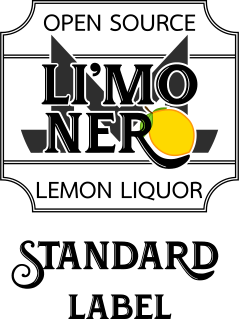
\includegraphics[width=1\textwidth]{img/std-label.pdf}
\end{center}

\begin{center}
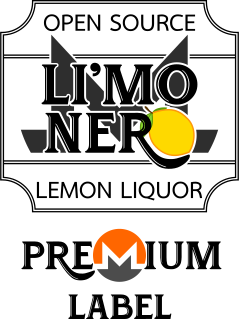
\includegraphics[width=1\textwidth]{img/prm-label.pdf}
\end{center}

\end{document}